\documentclass[border=6pt]{standalone}
\usepackage{tikz}
\usepackage{pgfplots}
\pgfplotsset{compat=1.18}
\usetikzlibrary{arrows.meta,positioning,shapes.geometric,fit,backgrounds,calc,decorations.pathreplacing,patterns,pgfplots.groupplots}
\tikzset{
  blk/.style={rectangle, rounded corners=2pt, draw=black!70, thick, fill=blue!6,
              minimum height=8mm, minimum width=20mm, align=center, font=\small},
  io/.style={rectangle, rounded corners=6pt, draw=black!70, thick, fill=green!8,
             minimum height=8mm, align=center, font=\small},
  proc/.style={rectangle, draw=black!70, thick, fill=orange!10, minimum height=8mm,
               align=center, font=\small},
  dec/.style={diamond, aspect=2, draw=black!70, thick, fill=yellow!15, align=center, font=\footnotesize},
  warnbox/.style={rectangle, rounded corners=2pt, draw=red!60!black, thick, fill=red!7,
                  minimum height=8mm, align=center, font=\small},
  oklbox/.style={rectangle, rounded corners=2pt, draw=green!45!black, thick, fill=green!8,
                 minimum height=8mm, align=center, font=\small},
  ar/.style={-{Latex[length=2mm]}, thick},
  arl/.style={-{Latex[length=2mm]}, thick, dashed, draw=black!55},
  lbl/.style={font=\footnotesize\itshape, text=black!60},
}
\definecolor{good}{RGB}{34,139,34}
\definecolor{bad}{RGB}{178,34,34}
\definecolor{warn}{RGB}{218,165,32}
\definecolor{pesblue}{RGB}{0,45,98}
\definecolor{complete}{RGB}{30,125,79}
\definecolor{partial}{RGB}{176,106,0}
\definecolor{blocked}{RGB}{166,43,43}
% ---------------------------------------------------------------------------
% figure-local styles
% ---------------------------------------------------------------------------
\pgfdeclarepatternformonly{hatchv}{\pgfqpoint{-1pt}{-1pt}}{\pgfqpoint{3pt}{3pt}}{\pgfqpoint{3pt}{3pt}}%
  {\pgfsetlinewidth{0.4pt}\pgfpathmoveto{\pgfqpoint{0pt}{0pt}}\pgfpathlineto{\pgfqpoint{0pt}{3pt}}%
   \pgfusepath{stroke}}
\tikzset{
  pnl/.style={rounded corners=3pt, thick},
  pnla/.style={pnl, draw=complete!85!black, fill=complete!5},
  pnlb/.style={pnl, draw=blocked!85!black, fill=blocked!5},
  prmpt/.style={rectangle, rounded corners=2pt, draw=black!70, thick, fill=blue!6,
                font=\footnotesize, inner sep=3.5pt, text width=6.4cm, align=center},
  cnt/.style={font=\scriptsize\itshape, text=black!65, align=center},
  comp/.style={rectangle, rounded corners=1pt, draw=black!55, thick, fill=black!4,
               minimum width=5.4mm, minimum height=5.0mm, inner sep=0pt,
               font=\scriptsize, align=center},
  chip/.style={rectangle, rounded corners=1pt, thick, minimum width=5.4mm,
               minimum height=5.0mm, inner sep=0pt, font=\scriptsize, align=center},
  chipgood/.style={chip, draw=good, fill=good!16},
  chipbad/.style={chip, draw=bad, fill=bad!13},
  stat/.style={rectangle, rounded corners=2pt, draw=black!55, thick, fill=white,
               font=\scriptsize, inner sep=4pt, text width=6.1cm, align=center},
  verd/.style={rectangle, rounded corners=2pt, thick, font=\footnotesize,
               inner sep=4pt, text width=6.3cm, align=left},
  verdg/.style={verd, draw=complete!85!black, fill=complete!10},
  verdr/.style={verd, draw=blocked!85!black, fill=blocked!10},
  hdrg/.style={font=\footnotesize\bfseries, text=complete!75!black},
  hdrr/.style={font=\footnotesize\bfseries, text=blocked!75!black},
}
\begin{document}
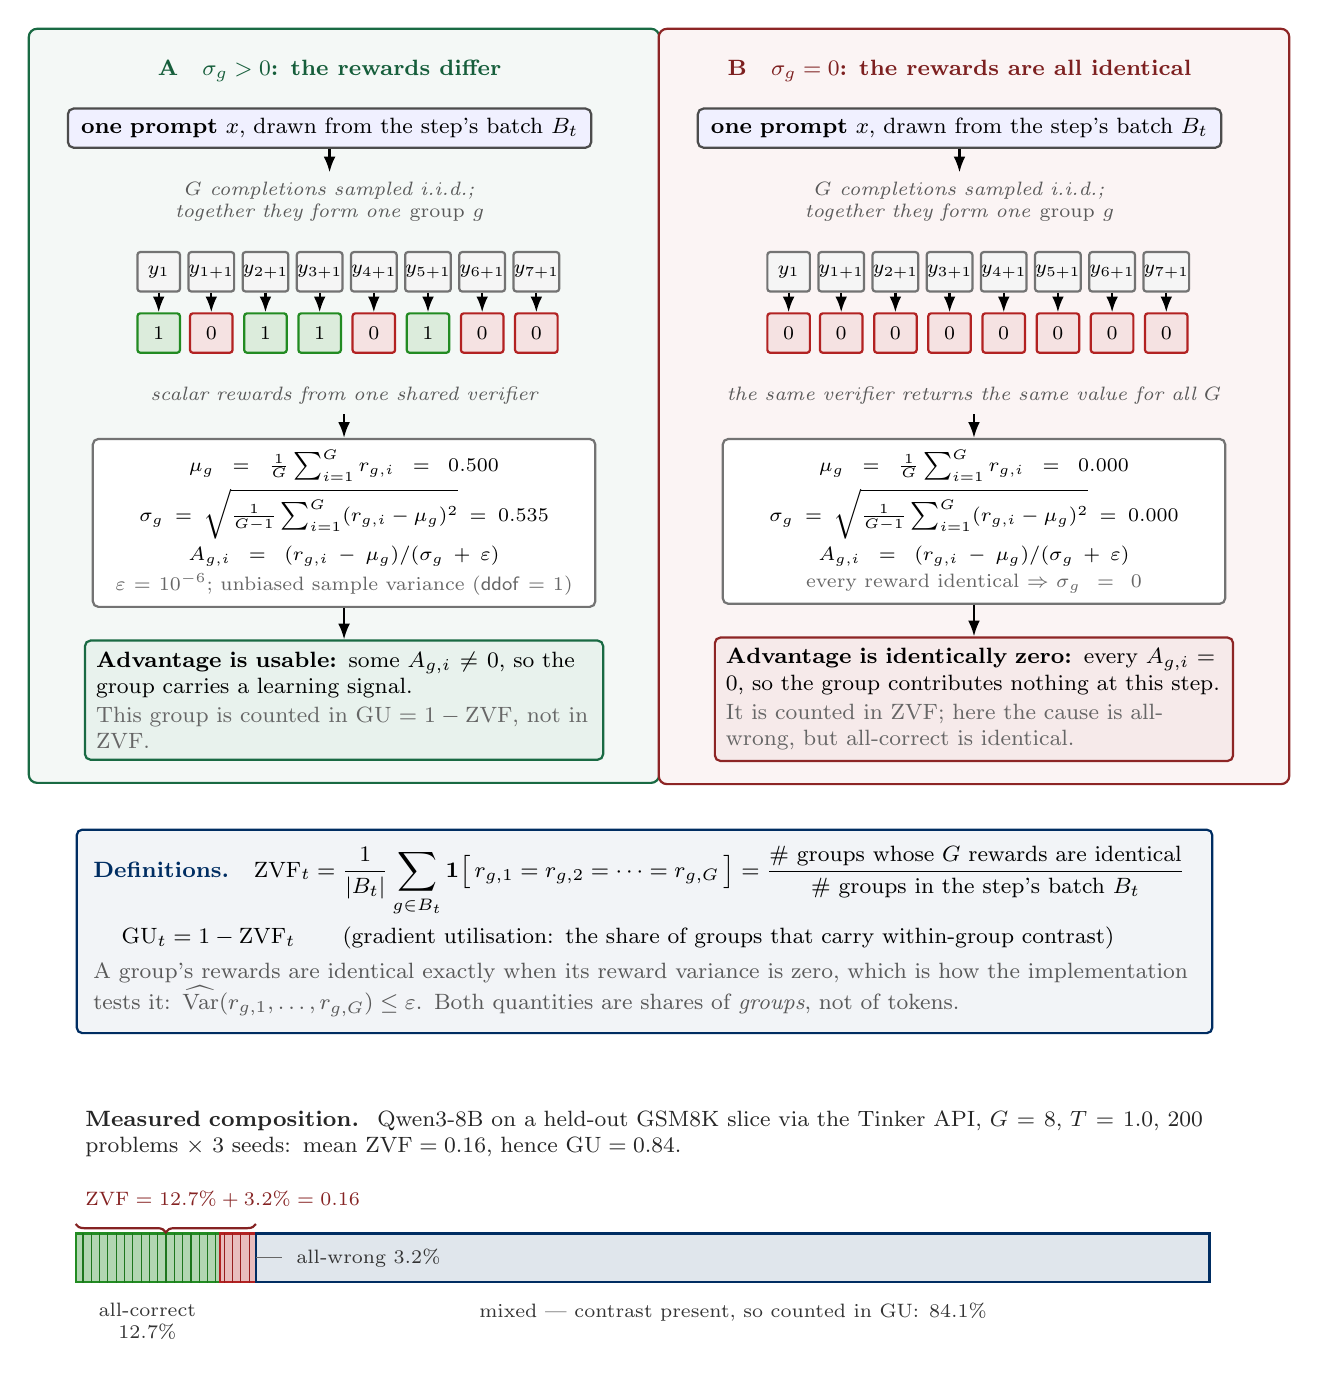
\begin{tikzpicture}

% ===========================================================================
% PANEL A --- rewards vary: within-group variance > 0, advantage is usable
% ===========================================================================
\begin{scope}[shift={(-4.00,0)}]
  \node[hdrg] (hA) at (0,0) {\textbf{A}\;\; $\sigma_g>0$: the rewards differ};

  \node[prmpt, below=2mm of hA] (PA)
    {\textbf{one prompt} $x$, drawn from the step's batch $B_t$};

  \node[cnt, text width=6.6cm, below=3mm of PA] (capA)
    {$G$ completions sampled i.i.d.;\\ together they form one \emph{group} $g$};
  \draw[ar] (PA.south) -- (capA.north);

  % 8 columns; each completion carries its own scalar reward directly beneath it
  \node[comp, below=2.5mm of capA, xshift=-2.17cm] (cA0) {$y_1$};
  \foreach \k in {1,2,3,4,5,6,7}{
    \pgfmathsetmacro{\km}{\k-1}
    \node[comp, right=0.8mm of cA\km] (cA\k) {$y_{\k+1}$};
  }
  \foreach \k/\v in {0/1,1/0,2/1,3/1,4/0,5/1,6/0,7/0}{
    \ifnum\v=1 \node[chipgood, below=2.5mm of cA\k] (rA\k) {\v}; \fi
    \ifnum\v=0 \node[chipbad,  below=2.5mm of cA\k] (rA\k) {\v}; \fi
    \draw[ar] (cA\k.south) -- (rA\k.north);
  }

  \node[cnt, text width=7.2cm, below=3mm of rA3, xshift=0.31cm] (cap2A)
    {scalar rewards from one shared verifier};

  \node[stat, below=3mm of cap2A] (SA)
    {$\mu_g=\frac{1}{G}\sum_{i=1}^{G} r_{g,i}=0.500$\\[1.5pt]
     $\sigma_g=\sqrt{\frac{1}{G-1}\sum_{i=1}^{G}(r_{g,i}-\mu_g)^2}=0.535$\\[1.5pt]
     $A_{g,i}=(r_{g,i}-\mu_g)/(\sigma_g+\varepsilon)$\\[1.5pt]
     \textcolor{black!60}{$\varepsilon=10^{-6}$; unbiased sample variance
      ($\mathsf{ddof}=1$)}};
  \draw[ar] (cap2A.south) -- (SA.north);

  \node[verdg, below=4mm of SA] (VA)
    {\textbf{Advantage is usable:} some $A_{g,i}\neq 0$, so the group carries a
     learning signal.\\[1pt]
     \textcolor{black!60}{This group is counted in
     $\mathrm{GU}=1-\mathrm{ZVF}$, not in $\mathrm{ZVF}$.}};
  \draw[ar] (SA.south) -- (VA.north);

  \begin{scope}[on background layer]
    \node[pnla, fit=(hA)(PA)(capA)(rA0)(rA7)(cap2A)(SA)(VA), inner sep=0.28cm] (pnlA) {};
  \end{scope}
\end{scope}

% ===========================================================================
% PANEL B --- rewards identical: within-group variance = 0, advantage is zero
% ===========================================================================
\begin{scope}[shift={(4.00,0)}]
  \node[hdrr] (hB) at (0,0) {\textbf{B}\;\; $\sigma_g=0$: the rewards are all identical};

  \node[prmpt, below=2mm of hB] (PB)
    {\textbf{one prompt} $x$, drawn from the step's batch $B_t$};

  \node[cnt, text width=6.6cm, below=3mm of PB] (capB)
    {$G$ completions sampled i.i.d.;\\ together they form one \emph{group} $g$};
  \draw[ar] (PB.south) -- (capB.north);

  \node[comp, below=2.5mm of capB, xshift=-2.17cm] (cB0) {$y_1$};
  \foreach \k in {1,2,3,4,5,6,7}{
    \pgfmathsetmacro{\km}{\k-1}
    \node[comp, right=0.8mm of cB\km] (cB\k) {$y_{\k+1}$};
  }
  \foreach \k in {0,1,2,3,4,5,6,7}{
    \node[chipbad, below=2.5mm of cB\k] (rB\k) {0};
    \draw[ar] (cB\k.south) -- (rB\k.north);
  }

  \node[cnt, text width=7.2cm, below=3mm of rB3, xshift=0.31cm] (cap2B)
    {the same verifier returns the same value for all $G$};

  \node[stat, below=3mm of cap2B] (SB)
    {$\mu_g=\frac{1}{G}\sum_{i=1}^{G} r_{g,i}=0.000$\\[1.5pt]
     $\sigma_g=\sqrt{\frac{1}{G-1}\sum_{i=1}^{G}(r_{g,i}-\mu_g)^2}=0.000$\\[1.5pt]
     $A_{g,i}=(r_{g,i}-\mu_g)/(\sigma_g+\varepsilon)$\\[1.5pt]
     \textcolor{black!60}{every reward identical $\Rightarrow$ $\sigma_g=0$}};
  \draw[ar] (cap2B.south) -- (SB.north);

  \node[verdr, below=4mm of SB] (VB)
    {\textbf{Advantage is identically zero:} every $A_{g,i}=0$, so the group
     contributes nothing at this step.\\[1pt]
     \textcolor{black!60}{It is counted in $\mathrm{ZVF}$; here the cause is
     all-wrong, but all-correct is identical.}};
  \draw[ar] (SB.south) -- (VB.north);

  \begin{scope}[on background layer]
    \node[pnlb, fit=(hB)(PB)(capB)(rB0)(rB7)(cap2B)(SB)(VB), inner sep=0.28cm] (pnlB) {};
  \end{scope}
\end{scope}

% ===========================================================================
% DEFINITIONS --- placed below whichever panel is deeper, so they cannot collide
% ===========================================================================
\path let \p1=(pnlA.south), \p2=(pnlB.south) in
  node[rectangle, rounded corners=2pt, draw=pesblue, thick, fill=pesblue!5,
       inner sep=6pt, font=\footnotesize, text width=14.0cm, align=left,
       anchor=north] (eqs) at (0,{min(\y1,\y2)-0.55cm})
  {\textbf{\textcolor{pesblue}{Definitions.}}\;\;
   $\displaystyle
     \mathrm{ZVF}_t=\frac{1}{|B_t|}\sum_{g\in B_t}
     \mathbf{1}\!\left[\,r_{g,1}=r_{g,2}=\cdots=r_{g,G}\,\right]
     =\frac{\mbox{\# groups whose $G$ rewards are identical}}
            {\mbox{\# groups in the step's batch $B_t$}}
   $\\[3pt]
   \hspace*{1.2em}$\displaystyle
     \mathrm{GU}_t=1-\mathrm{ZVF}_t
     \qquad\mbox{(gradient utilisation: the share of groups that carry
     within-group contrast)}$\\[3pt]
   \textcolor{black!65}{A group's rewards are identical exactly when its reward
   variance is zero, which is how the implementation tests it:
   $\widehat{\mathrm{Var}}(r_{g,1},\dots,r_{g,G})\le\varepsilon$. Both
   quantities are shares of \emph{groups}, not of tokens.}};

% ===========================================================================
% MEASURED COMPOSITION --- anchored to the definitions box, so it cannot collide
% ===========================================================================
\begin{scope}[shift={([yshift=-0.85cm]eqs.south west)}]
  \node[font=\footnotesize, text=black!85, align=left, text width=14.4cm,
        anchor=north west] at (0,0)
    {\textbf{Measured composition.}\; Qwen3-8B on a held-out GSM8K slice via the
     Tinker API, $G=8$, $T=1.0$, $200$ problems $\times$ $3$ seeds:
     mean $\mathrm{ZVF}=0.16$, hence $\mathrm{GU}=0.84$.};

  % bar geometry: 1 percentage point = 0.144 cm, so a 14.4 cm bar is 100 %
  \pgfmathsetmacro{\sA}{1.829}     % 12.7 % all-correct
  \pgfmathsetmacro{\xB}{2.290}     % + 3.2 % all-wrong -> the ZVF share
  \pgfmathsetmacro{\xEnd}{14.40}   % 100 %

  \fill[good!35, draw=good, thick] (0,-2.30) rectangle (\sA,-1.68);
  \fill[bad!30, draw=bad, thick]   (\sA,-2.30) rectangle (\xB,-1.68);
  \fill[pesblue!12, draw=pesblue, thick] (\xB,-2.30) rectangle (\xEnd,-1.68);
  % hatch overlay: a redundant, non-colour encoding of the two ZVF segments
  \fill[pattern=hatchv, pattern color=good!85!black] (0,-2.30) rectangle (\sA,-1.68);
  \fill[pattern=hatchv, pattern color=bad!85!black]  (\sA,-2.30) rectangle (\xB,-1.68);

  % segment labels (leader line for the narrow all-wrong segment)
  \node[font=\scriptsize, text=black!80, anchor=north, align=center] at (0.91,-2.44)
    {all-correct\\ $12.7\%$};
  \draw[black!60, thin] (\xB,-1.99) -- (2.62,-1.99);
  \node[font=\scriptsize, text=black!80, anchor=west] at (2.68,-1.99)
    {all-wrong $3.2\%$};
  \node[font=\scriptsize, text=black!80, anchor=north, align=center] at (8.35,-2.44)
    {mixed --- contrast present, so counted in $\mathrm{GU}$: $84.1\%$};

  % brace marking the ZVF portion of the bar
  \draw[decorate, decoration={brace, amplitude=3pt, mirror}, thick, draw=blocked!80!black]
    (0,-1.56) -- (\xB,-1.56);
  \node[font=\scriptsize, text=blocked!80!black, anchor=south west] at (0,-1.48)
    {$\mathrm{ZVF}=12.7\%+3.2\%=0.16$};
\end{scope}

\end{tikzpicture}
\end{document}
